\documentclass[uct_visualisation_thesis.tex]{subfiles}

\section{Architektura i działanie systemu}
\subsection{Wykorzystane technologie}
W naszym projekcie zdecydowaliśmy się skorzystać z technologii wymienionych poniżej.
\begin{enumerate}
	\item Języka \textit{Python} w wersji 3.7.2, który jest udostępniany na licencji \textit{GNU General Public License}.
	\item Biblioteki \textit{VisPy} w wersji 0.6.3, która udostępnia komponenty związane z wizualizacją graficzną. Wykorzystujemy tę bibliotekę w połączeniu z \textit{OpenGL} w wersji 2.1. Biblioteka \textit{VisPy} jest stworzona w oparciu o licencję \textit{BSD}, co w kontekście projektu na pracę inżynierską pozwala na modyfikowanie i wykorzystywanie jej.
	\item Biblioteki \textit{NumPy} w wersji  1.18.1, która odpowiada za wydajne operacje na macierzach. Zgodnie z umową licencyjną opisaną przez autorów \textit{NumPy}, można wykorzystywać ich narzędzie w zakresie pracy naukowej.
	\item Nakładki na bibliotekę \textit{Qt} - \textit{PyQt} w wersji 5.9.2. \textit{PyQt} umożliwia tworzenie interfejsu graficznego. Dla projektów takich jak praca inżynierska, \textit{PyQt} dystrybuowana jest na zasadach \textit{GNU General Public License}.
	\item Biblioteki \textit{fman build system (fbs)} w wersji 0.8.4, ułatwiającej pakowanie aplikacji korzystających z biblioteki \textit{PyQt} w celu stworzenia pliku instalacyjnego. To oprogramowanie dystrybuowane jest na zasadach \textit{GNU General Public License}.
	\item Narzędzia \textit{pdoc} w wersji 0.3.2, służącego do automatycznego generowania dokumentacji aplikacji. Zgodnie z umową licencyjną opisaną przez autorów \textit{pdoc}, można wykorzystywać ich narzędzie bez ograniczeń.
\end{enumerate}


\subsection{Wstęp}
Aplikacja jest podzielona na pięć oddzielnych modułów: \textit{Algorytm}, \textit{Serializacja}, \textit{Wizualizacja} i \textit{Gry}, które będą funkcjonować w obrębie nadrzędnego modułu - \textit{Aplikacji głównej}. Cele każdego z modułów i zadania powierzone im są przedstawione w rozdziałach \ref{subsec:algorithm} - \ref{subsec:mainapp}.


\subsection{Algorytm} \label{subsec:algorithm}
Moduł \textit{Algorytm} jest implementacją metody MCTS, korzystającą z wariantu UCT. Odpowiedzialnością tego modułu jest wyznaczanie kolejnego ruchu na podstawie dostarczonego stanu gry. Opisywany moduł będzie odpowiadał za iteracyjne tworzenie drzewa stanów i przeszukiwanie go w celu wyznaczenia najbardziej korzystnego ruchu. Użytkownik będzie miał możliwość zmiany liczby iteracji algorytmu albo ograniczenie czasowe jego działania.\\

W listingu \ref{lst:mcts}, opisującym zaimplementowany algorytm, operujemy na trzech istotnych zmiennych - \textit{tree}, \textit{curr\textunderscore node} i \textit{curr\textunderscore state}. Odpowiedzialnością struktury opisującej drzewo - \textit{tree} - jest przechowywanie korzenia oraz stanu wyjściowego rozgrywki, który jest tej samej struktury co zmienna \textit{curr\textunderscore state}. Struktura opisująca wierzchołek -- \textit{curr\textunderscore node} -- przechowuje wszystkie informacje na temat wierzchołka drzewa, wraz z referencjami do wierzchołków potomnych i rodzica. Dokładne relacje między komponentami zostały opisane na diagramie \ref{rys:umldiagram}.


\subsection{Serializacja} \label{subsec:serialization}
\textit{Serializacja} jest modułem odpowiadającym za zapisywanie drzew do plików formacie binarnym lub CSV. Pliki z drzewami w formacie binarnym mają umowne rozszerzenie \textit{.tree}. Oba schematy są rekurencyjne, bo taka jest również struktura generowanych przez aplikację drzew. To oznacza, że w celu zapisania całego drzewa, wystarczy przekazać odpowiednim komponentom jego korzeń.\\

\textbf{\large Serializacja binarna} \\
W serializacji binarnej przyjmujemy opisany niżej schemat.

\begin{itemize}
	\item \textbf{liczba całkowita} - wartość liczby zakodowanej w U2 na 4 bajtach. Bajty liczby w kolejności little endian.
	\item \textbf{napis}:
	\begin{itemize}
		\item liczba bajtów w napisie \textit{(liczba całkowita)},
		\item zawartość napisu kodowana w UTF-8.
	\end{itemize}
	\item \textbf{liczba zmiennoprzecinkowa} - wartość liczby zakodowanej w IEEE754 na 64 bitach w kolejności little endian.
	\item \textbf{wierzchołek:}
	\begin{itemize}
		\item nazwa stanu \textit{(napis)},
		\item $m$ - liczba węzłów potomnych \textit{(liczba całkowita)},
		\item $m$ powtórzeń następującego bytu:
		\begin{itemize}
			\item nazwa ruchu \textit{(napis)},
			\item licznik odwiedzin \textit{(liczba całkowita)},
			\item dodatkowy licznik odwiedzin \textit{(liczba całkowita)},
			\item średnia wypłata \textit{(liczba zmiennoprzecinkowa)},
			\item węzeł potomny \textit{(wierzchołek)}.
		\end{itemize}
	\end{itemize}
\end{itemize}


\textbf{\large Serializacja do plików csv} \\
W serializacji do plików csv przyjmujemy, że każdy kolejny wiersz odpowiada kolejnemu wierzchołkowi drzewa, a kolejne wartości opisujące wierzchołek oddzielamy przecinkami. Ostatnią wartością jest liczba wierzchołków potomnych. Każdy wierzchołek serializujemy do wiersza postaci:

\begin{center}
	\textbf{R, O, O2, W, S, D}
\end{center}
Oznaczenia:
\begin{itemize}
	\item R - nazwa ruchu,
	\item O - licznik odwiedzin,
	\item O2 - dodatkowy licznik odwiedzin,
	\item W - średnia wypłata algorytmu za ruch,
	\item S - nawa stanu,
	\item D - liczba wierzchołków potomnych.
\end{itemize}

Kolejność wierszy opisujących wierzchołki jest analogiczna do odwiedzania wierzchołków przez algorytm przeszukiwania drzewa wgłąb, począwszy od korzenia.

\begin{itemize}
	\item Jeśli wierzchołek $v$ ma jednego potomka $v_1$, to wiersz opisujący $v_1$ znajduje się pod wierszem opisującym $v$.
	\item Jeśli wierzchołek $v$ ma $n$ potomków $v_1, v_2, ..., v_n$ i żaden z potomków nie ma swoich potomków, to pod wierszem opisującym $v$ kolejne $n$ wierszy opisuje wierzchołki $v_1, v_2, ..., v_n$.
\end{itemize}


\subsection{Wizualizacja}
Moduł \textit{Wizualizacja} udostępnia funkcjonalność wizualizacji dostarczonych drzew. \textit{Wizualizacja} jest jedynym modułem, który korzysta z technologii \textit{VisPy} oraz \textit{NumPy}. Wykorzystanie tych technologii ma na celu odpowiednio wydajne wyświetlenie wizualizacji oraz przechowywanie wektorów z danymi, które będzie można przekazać karcie graficznej. Zadania \textit{Wizualizacji} są wymienione poniżej.

\begin{itemize}
	\item Przypisanie wierzchołkom drzewa miejsce na płaszczyźnie przy użyciu usprawnionego algorytmu Walkera i przetransformowanie wyznaczonych koordynatów do układu współrzędnych OpenGL.
	\item Przypisanie krawędziom koloru w zależności od liczby odwiedzin wierzchołka.
	\item Przypisanie wierzchołkom koloru w zależności od gracza reprezentowanego stanu gry.
	\item Detekcja kliknięcia wierzchołka przez użytkownika.
	\item Wyświetlenie drzewa.
	\item Przybliżanie, oddalanie i poruszanie się po wizualizacji.
\end{itemize}


\subsection{Gry}
Prezentowane rozwiązanie udostępnia dwie gry planszowe w ramach modułu \textit{Gry}. System został przygotowany z myślą o rozszerzaniu o kolejne gry. Wymagania, które należy spełnić, dodając kolejną grę, są opisane w rozdziale \ref{subsec:uml}.


\subsection{Aplikacja główna} \label{subsec:mainapp}
\textit{Aplikacja główna} jest modułem łączącym wszystkie pozostałe. Ten moduł skupia się na zaprezentowaniu funkcjonalności wszystkich modułów w formie aplikacji okienkowej. Interfejsy, które udostępnia \textit{Aplikacja główna}, są opisane w rozdziale \ref{sec:ui}.


\section{Główne komponenty aplikacji}
\subsection{Diagram klas} \label{subsec:uml}
Klasa \textit{MonteCarloNode}, zgodnie z diagramem \ref{rys:umldiagram_node}, reprezentuje wierzchołek w drzewie, więc przechowuje referencje do swojego rodzica i wierzchołków potomnych, aby zachować rekurencyjną strukturę drzewa. Ponadto zawiera wszystkie informacje związane z przebiegiem algorytmu UCT w polu \textit{details} oraz algorytmu Walkera w polu \textit{vis\textunderscore details}.

\begin{figure}[h!]
	\centering
	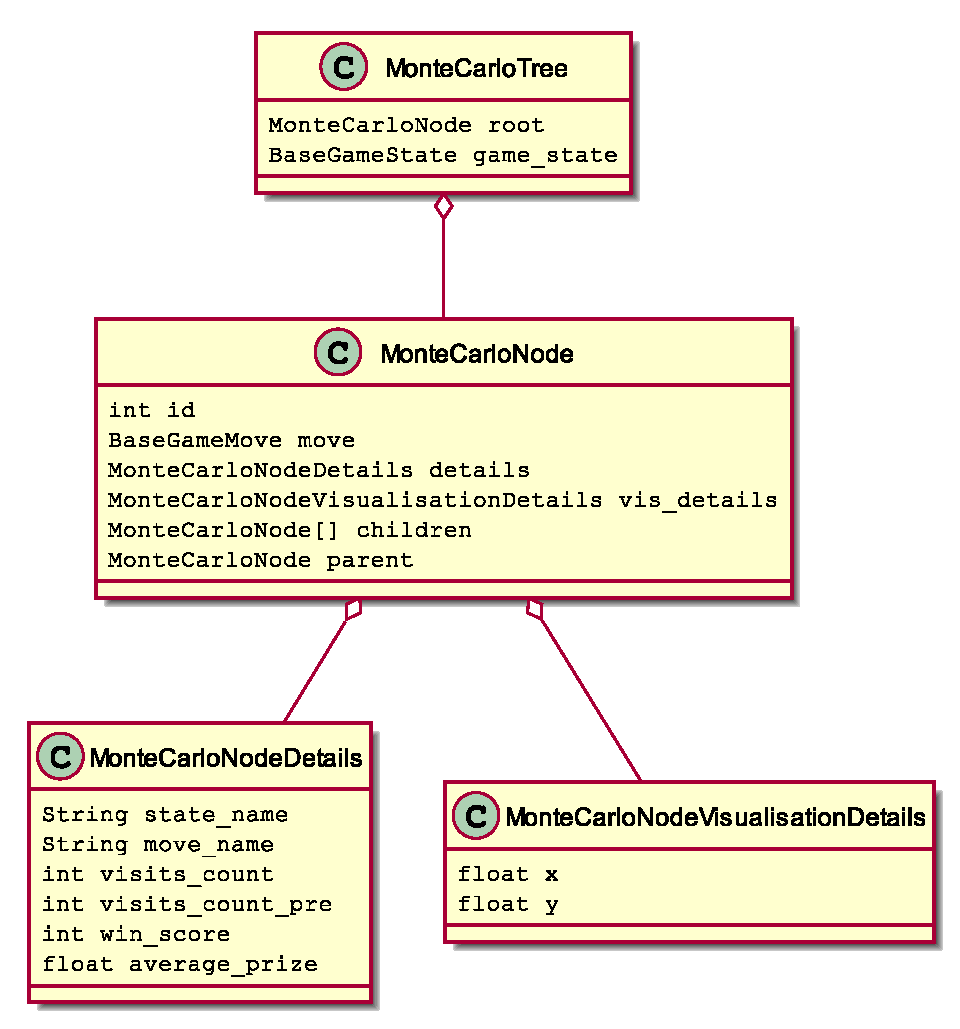
\includegraphics[width=0.5\linewidth]{umldiagram_node}
	\caption{Diagram UML klasy wierzchołka}
	\label{rys:umldiagram_node}
\end{figure}

Diagram \ref{rys:umldiagram_algorithm} ukazuje najistotniejsze klasy modułu \textit{Algorytm}. Metoda \textit{calculate\textunderscore next\textunderscore move} klasy \textit{MonteCarloTreeSearch} odpowiada za wykonanie kolejnych iteracji algorytmu. Algorytm zapisuje informacje o rozgrywanych playoutach w polach klasy \textit{MonteCarloNodeDetails} analizowanych wierzchołków. Ruch oraz stan analizowanej gry są opisane odpowiednio przez klasy \textit{GameMove} i \textit{GameState}. Implementacja metod tych klas daje możliwość łatwego rozszerzenia aplikacji o inne gry. Istotny z punktu widzenia konstrukcji drzewa jest stan rozgrywki, który opisują pola typu wyliczeniowego \textit{GamePhase}.

\begin{figure}[h!]
	\centering
	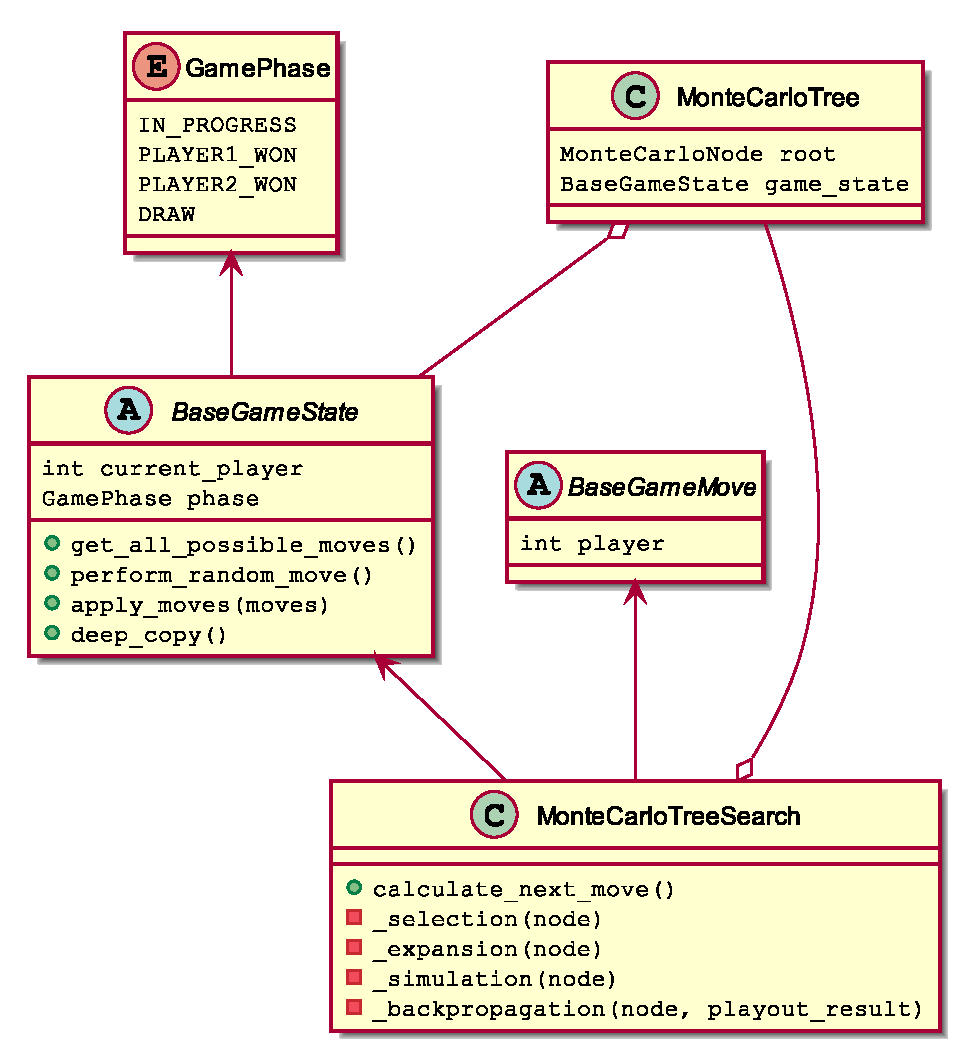
\includegraphics[width=0.5\linewidth]{umldiagram_algorithm}
	\caption{Diagram UML dla modułu \textit{Algorytm}}
	\label{rys:umldiagram_algorithm}
\end{figure}

Zgodnie z diagramami \ref{rys:umldiagram_serialization_visualisation} i \ref{rys:umldiagram_algorithm}, klasy \textit{MonteCarloTreeSearch}, \textit{ImprovedWalkersAlgorithm} oraz \textit{Serializator} są pośrednio lub bezpośrednie zależne od klasy \textit{MonteCarloNode}, opisującej wierzchołek w drzewie. Jest to część wspólna modułów \textit{Algorytm}, \textit{Wizualizacja} i \textit{Serializacja}.

\begin{figure}[h!]
	\centering
	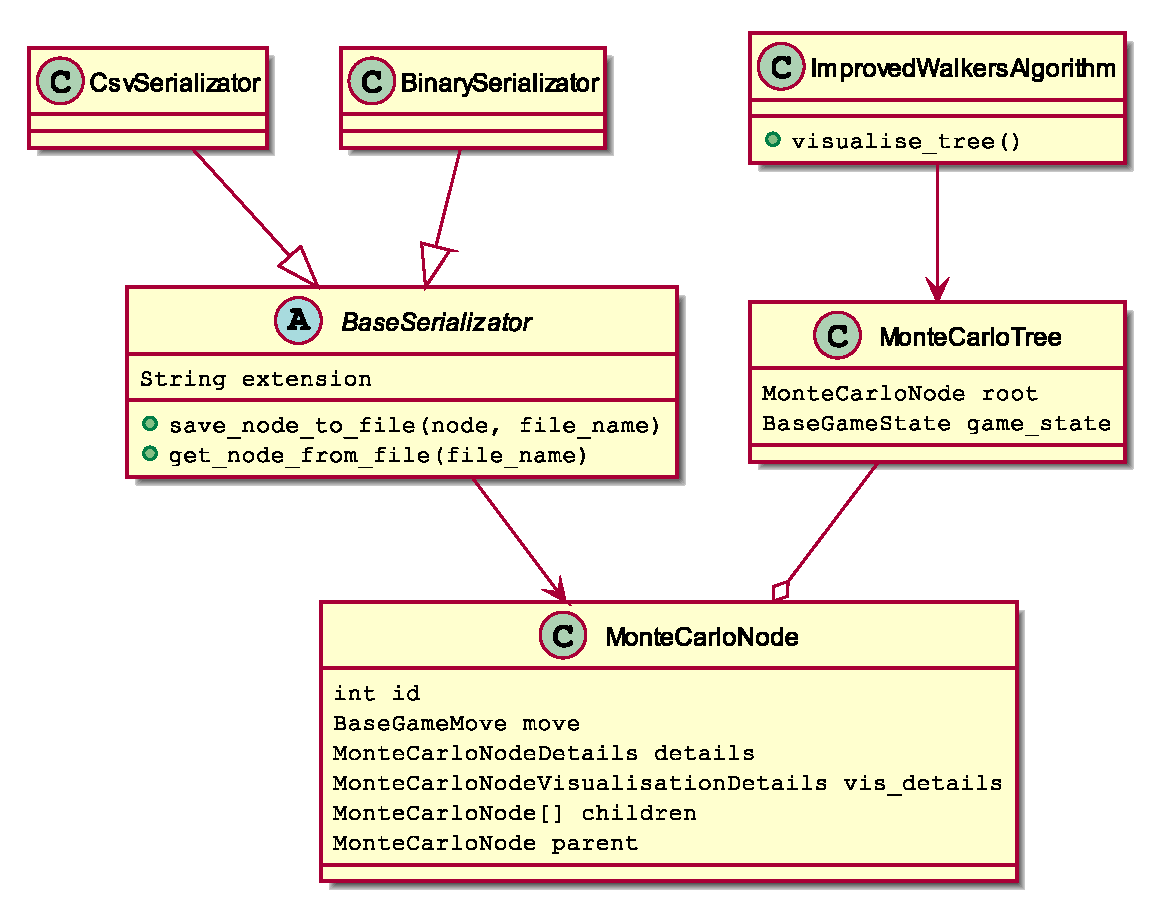
\includegraphics[width=0.6\linewidth]{umldiagram_serialization_visualisation}
	\caption{Diagram UML dla modułów \textit{Serializacja} i \textit{Wizualizacja}}
	\label{rys:umldiagram_serialization_visualisation}
\end{figure}

Widniejąca na diagramie \ref{rys:umldiagram_serialization_visualisation} klasa \textit{ImprovedWalkersAlgorithm} jest głównym komponentem modułu \textit{Wizualizacja}. Jego odpowiedzialnością jest wyznaczenie układu wierzchołków drzewa na płaszczyźnie. Szczegóły związane z przebiegiem algorytmu Walkera i rysowaniem każdego wierzchołka, zawarte są w polach klasy \textit{MonteCarloVisualisationDetails}. \textit{Serializator} jest klasą opisującą funkcjonalności, które mają udostępnić właściwe implementacje serializatorów, czyli serializowanie drzew do plików oraz deserializację z plików.
